\documentclass[14pt]{extarticle}
\usepackage{graphicx} 
\usepackage{float} 
\usepackage{color}
\usepackage[a4paper, total={6in, 8in},left=2cm,right=2cm,
top=2cm,bottom=2cm,bindingoffset=0cm]{geometry}
\usepackage[utf8]{inputenc}
\usepackage[english, russian]{babel}
\usepackage{amsmath}
\usepackage{amsfonts}
\usepackage[colorlinks = true, allcolors = cyan]{hyperref}
\usepackage{xfrac}
\usepackage{indentfirst}
\graphicspath{ {./images/} }
\newenvironment{comment}{}{}

\newcommand{\RomanNumeralCaps}[1]
    {\MakeUppercase{\romannumeral #1}}

\DeclareMathOperator{\med}{med} %Медиана
\DeclareMathOperator{\pirs}{r} %Коэффициент корреляции Пирсона
\DeclareMathOperator{\sign}{sign} %Сигнум-функция

\begin{document}

\begin{titlepage}

\begin{center}
    Санкт-Петербургский политехнический университет \\Петра Великого
\end{center}

\begin{center}
    Физико-механический институт
\end{center}

\begin{center}
    Высшая школа прикладной математики и вычислительной\\ физики
\end{center}

\vspace{8em}

\begin{center}
\rule{\textwidth}{1pt} 
\\
\textbf{Отчёт\\
по лабораторным работам №1-4\\
по дисциплине\\
<<Математическая статистика>>}
\rule{\textwidth}{1pt} 
\\
\end{center}

\vspace{8em}


\begin{flushright}
\begin{minipage}{.45\textwidth}
Выполнил студент:\\
Тасаков Антон Павлович\\
группа:\\
5030102/10201\\
Проверил:\\
доцент\\
Баженов Александр Николаевич
\end{minipage}
\end{flushright}

\vspace{8em}
\begin{center}
    Санкт-Петербург\\
    2024
\end{center}

\end{titlepage}

\tableofcontents
\newpage
\listoffigures
\newpage
\listoftables
\newpage
\section{Постановка задачи}

\subsection{Часть 1}
Для 5 распределений:
\begin{itemize}
    \item Нормальное распределение $N(x, 0, 1)$
    \item распределение Коши $C(x, 0, 1)$
    \item Распределение Стьюдента $t(x, 0, 3)$ с тремя степенями свободы
    \item Распределение Пуассона $P(k, 10)$
    \item Равномерное распределение $U(x, -\sqrt3, \sqrt3)$
\end{itemize}
Сгенерировать выборки размером 10, 50, 1000 элементов.\\
Построить на одном рисунке гистограмму и график плотности распределения.

\subsection{Часть 2}
Сгенерировать выборки размером 10, 100, 1000 элементов.\\
Для каждой выборки вычислить следующие статистические характеристики положения данных: $\overline{x}$, $med\:x$, $z_{Q}$, $z_{R}$, $z_{tr}$. Повторить такие вычисления 1000 раз для каждой выборки и найти среднее характеристик положения и их квадратов: $E(z) = \bar{z}$. Вычислить оценку дисперсии по формуле $D(z) = \overline{z^2} - \overline{z}^2$.

\subsection{Часть 3}
Для данных распределений сгенерировать выборки размером 20 и 100 элементов. Построить для них боксплот Тьюки.

\subsection{Часть 4}
Для данных распределений сгенерировать выборки размером 20 и 100 элементов. Вычислить параметры положения и рассеяния. Представить результаты графически.


\section{Теория}
\subsection{Функции распределения}
\begin{itemize}
    \item Нормальное распределение 
    \begin{equation}
        N(x, 0, 1) = \frac{1}{\sqrt{2\pi}}e^\frac{-x^2}{2}
        \label{eq1}
    \end{equation}
    
    \item Распределение Коши 
    \begin{equation}
       C(x, 0, 1) = \frac{1}{\pi}\frac{1}{x^2+1}
       \label{eq2}
    \end{equation}
    
    \item Распределение Стьюдента $t(x, 0, 3)$ с тремя степенями свободы
     \begin{equation}
       t(x, 0, 3) = \frac{6\sqrt3}{\pi(3 + t^2)^2}
       \label{eq3}
    \end{equation}
    
    \item Распределение Пуассона 
     \begin{equation}
       P(k, 10) = \frac{10^k}{k!}e^{-10}
       \label{eq4}
    \end{equation}
    
    \item Равномерное распределение 
     \begin{equation}
       U(x, -\sqrt3, \sqrt3) = \begin{cases}
       \frac{1}{2\sqrt3} & \mbox{при} \; |x| \leq \sqrt3\\
       0 & \mbox{при} \; |x| > \sqrt3
       \end{cases}
       \label{eq5}
    \end{equation}
    
\end{itemize}

\subsection{Характеристики положения}

\begin{itemize}
    \item Выборочное среднее
    \begin{equation}
        \overline{x} = \tfrac{1}{n}\sum_{i = 1}^{n}x_i
        \label{eq6}
    \end{equation}
    \item Выборочная медиана
    
       \begin{equation}
med\ x = \left\{
\begin{array}{ccl}
x_{(l + 1)} & \text{при} & n = 2l + 1\\
\dfrac{x_{(l)} + x_{(l + 1)}}{2} & \text{при} & n = 2l
\end{array}
\right.
\label{eq7}
\end{equation}
    
    \item Полусумма экстремальных выборочных элементов
    \begin{equation}
        z_{R} = \frac{x_{(1)} + x_{(n)}}{2}
        \label{eq8}
    \end{equation}
    \item Полусумма квартилей\\
    Выборочная квартиль $z_{p}$ порядка $p$ определяется формулой
    \begin{equation}
        z_{p} = \left\{
\begin{array}{ccl}
x_{([np]+ 1)} & \text{при} & np\ \text{дробном}\\
x_{(np)} & \text{при} & np\ \text{целом}
\end{array}
\right.
\label{eq9}
    \end{equation}
    Полусумма квартилей\\
    \begin{equation}
        z_{Q} = \dfrac{z_{1/4} + z_{3/4}}{2}
        \label{eq10}
    \end{equation}
    \item Усечённое среднее
    
    \begin{equation}
        z_{tr} = \tfrac{1}{n - 2r}\sum_{i = r + 1}^{n - r}x_{(i)},\ r\approx\dfrac{n}{4}
        \label{eq11}
    \end{equation}
    \item Оценка дисперсии
    \begin{equation}
        D(z) = \overline{z^2} - \overline{z}^2
        \label{eq12}
    \end{equation}
\end{itemize}

\subsection{Бокс-плот Тьюки}
Боксплот (англ. box plot) — график, использующийся в описательной статистике, компактно изображающий одномерное распределение вероятностей.
Такой вид диаграммы в удобной форме показывает медиану, нижний и верхний квартили и выбросы. Границами ящика служат первый и третий квартили, линия в середине ящика — медиана. Концы усов — края статистически
значимой выборки (без выбросов). Длину «усов» определяют разность первого квартиля и полутора межквартильных расстояний и сумма третьего
квартиля и полутора межквартильных расстояний. Формула имеет вид

\begin{equation}
    X_{1} = Q_{1} - \dfrac{3}{2}(Q_{3} -Q_{1}),\;\; X_{2} = Q_{3} + \dfrac{3}{2}(Q_{3} -Q_{1})
    \label{eq13}
\end{equation}

\noindentгде $X_{1}$ — нижняя граница уса, $X_{2}$ — верхняя граница уса, $Q_{1}$ — первый
квартиль, $Q_{3}$ — третий квартиль. Данные, выходящие за границы усов (выбросы), отображаются на графике в виде маленьких кружков.\\
Выбросами считаются величины $x$, такие что


\begin{equation}
    \left[
  \begin{array}{ccc}
        x < X_{1}^{T}\\
        x > X_{2}^{T}
  \end{array}
\right.
\label{eq14}
\end{equation}

\subsection{ Доверительные интервалы для параметров нормального распределения}

\subsubsection{Доверительный интервал для среднего значения m нормального распределения}

Дана выборка $(x_1, x_2, ... x_n)$ объёма $n$ из нормальной генеральной совокупности. На её основе строим выборочное среднее $\overline{x}$ и выборочное среднее квадратическоеп отклонение $s$. Параметры $m$ и $\sigma$ нормального распределения неизвестны.\\
Доказано, что случайная величина:
\begin{equation}
    T = \sqrt{n - 1}\cdot \dfrac{\overline{x} - m}{s}
    \label{eq15}
\end{equation}

\noindent называемая статистикой Стьюдента, распределена по закону Стьюдента с $n-1$ степенями свободы. Пусть $f_{T}(x)$ - плотность вероятности этого распределения. Тогда 

\begin{multline*}
    P(-x < \sqrt{n - 1}\cdot \dfrac{\overline{x} - m}{s} < x) = P(-x < \sqrt{n - 1}\cdot \dfrac{m - \overline{x}}{s} < x) = \\ =\int \limits_{-x}^{x}f_{T}(t)dt = 2\int \limits_{0}^{x}f_{T}(t)dt = 2\Bigg(\int \limits_{-\infty}^{x}f_{T}(t)dt - \dfrac{1}{2}\Bigg) = 2F_{T}(x) - 1
\end{multline*}

\noindent Здесь  $F_{T}(x)$ - функция распределения Стьюдента с $n-1$ степенями свободы.\\
Полагаем $2F_{T}(x) - 1 = 1 - \alpha$, где $\alpha$ - выбранный уровень значимости. Тогда $F_{T}(x) = 1 - \sfrac{\alpha}{2}$. Пусть $t_{1 - \sfrac{\alpha}{2}}(n-1)$ - квантиль распределения Стьюдента с $n-1$ степенями свободы и порядка $1 - \sfrac{\alpha}{2}$. Из предыдущих равенств получаем

\begin{multline}
    P(\overline{x} - \dfrac{sx}{\sqrt{n - 1}} < m < \overline{x} + \dfrac{sx}{\sqrt{n - 1}}) = 2F_{T}(x) - 1 = 1 - \alpha, \\
    P(\overline{x} - \dfrac{st_{1 - \sfrac{\alpha}{2}}(n-1)}{\sqrt{n - 1}} < m < \overline{x} + \dfrac{st_{1 - \sfrac{\alpha}{2}}(n-1)}{\sqrt{n - 1}}) = 1 - \alpha
    \label{eq16}
\end{multline}

 \noindent что и даёт доверительный интервал для $m$ с доверительной верятностью $\gamma = 1 - \alpha$. 
        






\subsubsection{Доверительный интервал для среднего квалратического отклонения нормального распределения}

Дана выборка $(x_1, x_2, ... x_n)$ объёма $n$ из нормальной генеральной совокупности. На её основе строим выборочную дисперсию $s^2$.Параметры $m$ и $\sigma$ нормального распределения неизвестны.\\
Доказано, что случайная величина $\sfrac{ns^2}{\sigma^2}$ распределена по закону $\chi^2$ с $n-1$ степенями свободы.\\
Задаёмся уровнем значимости $\alpha$ и по таблице находим квантили $\chi_{\sfrac{\alpha}{2}}^{2}(n-1)$ и $\chi_{1 - \sfrac{\alpha}{2}}^{2}(n-1)$. Это значит, что\\
\begin{center}
    $P(\chi^{2}(n - 1) < \chi_{\sfrac{\alpha}{2}}^{2}(n-1)) = \sfrac{\alpha}{2}\;\;\;\;
    P(\chi^{2}(n - 1) < \chi_{1 - \sfrac{\alpha}{2}}^{2}(n-1)) = 1 - \sfrac{\alpha}{2}$
\end{center}
\noindent Откуда можно получить, что 
\begin{equation}
    P\Bigg(\dfrac{s\sqrt{n}}{\sqrt{\chi_{1 - \sfrac{\alpha}{2}}^{2}(n-1)}} < \sigma < \dfrac{s\sqrt{n}}{\sqrt{\chi_{\sfrac{\alpha}{2}}^{2}(n-1)}}\Bigg) = 1 - \alpha
    \label{eq17}
\end{equation}

\noindent что и даёт доверительный интервал для $\sigma$ с с доверительной верятностью $\gamma = 1 - \alpha$. 



\subsubsection{Доверительный интервал для среднего значения m произвольной генеральной совокупности при большом объёме выборки}

Пусть 
\begin{equation*}
    \Phi(x) = \dfrac{1}{\sqrt{2\pi}} \int \limits_{-\infty}
 ^{x}e^{\sfrac{-t^2}{2}}dt
 \end{equation*}
\noindent - функция Лапласа. тогда
$$P\Bigg(-x < \sqrt{n}\cdot \dfrac{\overline{x} - m}{\sigma} < x\Bigg) \approx 2\Phi(x) - 1$$
\noindent Откуда 
$$P\Bigg(\overline{x} - \dfrac{\sigma x}{\sqrt{n}} < m < \overline{x} + \dfrac{\sigma x}{\sqrt{n}}\Bigg) \approx 2\Phi(x) - 1$$

\noindent Положим $2\Phi(x) - 1 = \gamma = 1 -\alpha$. Пусть $u_{1 - \sfrac{\alpha}{2}}$ - квантиль нормального распределения $N(0, 1)$ порядка $1 - \sfrac{\alpha}{2}$. Получим

\begin{equation}
    P\Bigg(\overline{x} - \dfrac{su_{1 - \sfrac{\alpha}{2}}}{\sqrt{n}} < m < \overline{x} + \dfrac{su_{1 - \sfrac{\alpha}{2}}}{\sqrt{n}}\Bigg) \approx \gamma
    \label{eq18}
\end{equation}

\noindent что и даёт доверительный интервал для $m$ с с доверительной верятностью $\gamma = 1 - \alpha$. 


\subsubsection{Доверительный интервал для среднего квадратического отклонения произвольной генеральной совокупности при большом объёме выборки}

Пусть 
\begin{equation*}
    \Phi(x) = \dfrac{1}{\sqrt{2\pi}} \int \limits_{-\infty}
 ^{x}e^{\sfrac{-t^2}{2}}dt
 \end{equation*}
\noindent - функция Лапласа. Тогда 
$$P\Bigg(-x < \dfrac{s^2 - Ms^2}{\sqrt{Ds^2}} < x\Bigg) \approx 2\Phi(x) - 1$$

\noindent Положим $2\Phi(x) - 1 = \gamma = 1 -\alpha$. Пусть $u_{1 - \sfrac{\alpha}{2}}$ - квантиль нормального распределения $N(0, 1)$ порядка $1 - \sfrac{\alpha}{2}$. Получим

$$\sqrt{Ds^2} \approx \dfrac{\sigma^2}{\sqrt{n}}\sqrt{e + 2} $$

\begin{equation}
    s(1 + u_{1 - \sfrac{\alpha}{2}}\sqrt{\sfrac{(e+2)}{n}})^{\sfrac{-1}{2}} < \sigma < s(1 - u_{1 - \sfrac{\alpha}{2}}\sqrt{\sfrac{(e+2)}{n}})^{\sfrac{-1}{2}}
    \label{eq19}
\end{equation}
\noindent что и даёт доверительный интервал для $\sigma$ с с доверительной верятностью $\gamma = 1 - \alpha$. 
\section{Описание работы}
Лабораторная работа выполнена на языке программирования R. C помощью встроенных средств языка были сгенерированы выборки значений для 5 распределений (\ref{eq1} - \ref{eq5}), построены требуемые графики (рис. \ref{fig1} - \ref{fig15}) и рассчитаны характеристики положения (таблицы \ref{table:1} - \ref{table:10}). Исходный код лабораторной работы: \url{https://github.com/Darknessich/Statistics/tree/master/Lab1/}

\section{Результаты}
\subsection{Гистограммы и графики плотности распределения}
\begin{figure}[H]
    \centering
    \includegraphics[width = 1\linewidth]{hist/normal.png}
    \caption{Нормальное распределение (\ref{eq1})}
    \label{fig1}
\end{figure}

\begin{figure}[H]
    \centering
    \includegraphics[width = 1\linewidth]{hist/cauchy.png}
    \caption{Распределение Коши (\ref{eq2})}
    \label{fig2}
\end{figure}

\begin{figure}[H]
    \centering
    \includegraphics[width = 1\linewidth]{hist/student.png}
    \caption{Распределение Стьюдента (\ref{eq3})}
    \label{fig3}
\end{figure}

\begin{figure}[H]
    \centering
    \includegraphics[width = 1\linewidth]{hist/poisson.png}
    \caption{Распределение Пуассона (\ref{eq4})}
    \label{fig4}
\end{figure}

\begin{figure}[H]
    \centering
    \includegraphics[width = 1\linewidth]{hist/uniform.png}
    \caption{Равномерное распределение (\ref{eq5})}
    \label{fig5}
\end{figure}

\subsection{Характеристики положения}

\begin{table}[H]
    \centering
    \begin{tabular}{ |c|c|c|c|c|c| } 
 \hline
 normal n = 10 & & & & & \\ 
 \hline
  &$\overline{x}\ (\ref{eq6})$ & $med\ x\ (\ref{eq7})$ & $z_{R}\ (\ref{eq8})$ & $z_{Q}\ (\ref{eq10})$ & $z_{tr}\ (\ref{eq11})$\\ 
 \hline
 $E(z)$ & $5,4 \cdot 10^{-3}$ & $-4,4\cdot 10^{-3}$ & $-1,2 \cdot 10^{-2}$ & $7,3 \cdot 10^{-3}$ & $2,4 \cdot 10^{-2}$ \\ 
 \hline
 $D(z)\ (\ref{eq12})$ & $3,2\cdot 10^{-1}$ & $3,7 \cdot 10^{-1}$ & $4,4 \cdot 10^{-1}$ & $3,5 \cdot 10^{-1}$ & $4,1 \cdot 10^{-1}$ \\ 
 \hline\hline
 normal n = 100 & & & & & \\
 \hline
 &$\overline{x}$ & $med\ x$ & $z_{R}$ & $z_{Q}$ & $z_{tr}$\\ 
 \hline
 $E(z)$ & $-1,7 \cdot 10^{-3}$ & $-2,0 \cdot 10^{-3}$ & $-1,1 \cdot 10^{-2}$ & $-1,3 \cdot 10^{-3}$ & $-2,6 \cdot 10^{-3}$ \\ 
 \hline
 $D(z)$ & $9,5 \cdot 10^{-2}$ & $1,2 \cdot 10^{-1}$ & $2,9 \cdot 10^{-1}$ & $1,1 \cdot 10^{-1}$ & $1,4 \cdot 10^{-1}$ \\ 
 \hline\hline
 normal n = 1000 & & & & & \\
 \hline
 &$\overline{x}$ & $med\ x$ & $z_{R}$ & $z_{Q}$ & $z_{tr}$\\ 
 \hline
 $E(z)$ & $-7,0 \cdot 10^{-4}$ & $-1,1 \cdot 10^{-3}$ & $-8,9 \cdot 10^{-3}$ & $0,0 $ & $5,0 \cdot 10^{-4}$ \\ 
 \hline
 $D(z)$ & $3,1 \cdot 10^{-2}$ & $4,0 \cdot 10^{-2}$ & $2,4 \cdot 10^{-1}$ & $3,4 \cdot 10^{-2}$ & $4,4 \cdot 10^{-2}$ \\
 \hline
\end{tabular}
    \caption{Нормальное распределение}
    \label{table:1}
\end{table}


\begin{table}[H]
    \centering
    \begin{tabular}{ |c|c|c|c|c|c| } 
 \hline
 cauchy n = 10 & & & & & \\ 
 \hline
  &$\overline{x}\ (\ref{eq6})$ & $med\ x\ (\ref{eq7})$ & $z_{R}\ (\ref{eq8})$ & $z_{Q}\ (\ref{eq10})$ & $z_{tr}\ (\ref{eq11})$\\ 
 \hline
 $E(z)$ & $3,1 \cdot 10^{-1}$ & $-6,7 \cdot 10^{-3}$ & $ 1,7 $ & $ -4,4 \cdot 10^{-2}$ & $-9,7 \cdot 10^{-1}$ \\ 
 \hline
 $D(z)\ (\ref{eq12})$ & $3,7 \cdot 10^{1}$ & $5,7 \cdot 10^{-1}$ & $1,8 \cdot 10^{2}$ & $9,5 \cdot 10^{-1}$ & $1,6 \cdot 10^{1}$ \\ 
 \hline\hline
 cauchy n = 100 & & & & & \\
 \hline
 &$\overline{x}$ & $med\ x$ & $z_{R}$ & $z_{Q}$ & $z_{tr}$\\ 
 \hline
 $E(z)$ & $1,3$ & $5,3 \cdot 10^{-3}$ & $6,6 \cdot 10^{1}$ & $3,1 \cdot 10^{-3}$ & $3,6$ \\ 
 \hline
 $D(z)$ & $5,2 \cdot 10^{1}$ & $1,6 \cdot 10^{-1}$ & $2,6 \cdot 10^{3}$ & $2,4 \cdot 10^{-1}$ & $8,9 \cdot 10^{1}$ \\ 
 \hline\hline
 cauchy n = 1000 & & & & & \\
 \hline
 &$\overline{x}$ & $med\ x$ & $z_{R}$ & $z_{Q}$ & $z_{tr}$\\ 
 \hline
 $E(z)$ & $-6,4$ & $3,7\cdot 10^{-3}$ & $-3,2 \cdot 10^{3}$ & $6,6 \cdot 10^{-3}$ & $-1,6$ \\ 
 \hline
 $D(z)$ & $1,8 \cdot 10^{2}$ & $5,0 \cdot 10^{-2}$ & $9,2 \cdot 10^{4}$ & $7,0 \cdot 10^{-2}$ & $2,9 \cdot 10^{1}$ \\
 \hline
\end{tabular}
    \caption{Распределение Коши}
    \label{table:2}
\end{table}


\begin{table}[H]
    \centering
    \begin{tabular}{ |c|c|c|c|c|c| } 
 \hline
 student n = 10 & & & & & \\ 
 \hline
  &$\overline{x}\ (\ref{eq6})$ & $med\ x\ (\ref{eq7})$ & $z_{R}\ (\ref{eq8})$ & $z_{Q}\ (\ref{eq10})$ & $z_{tr}\ (\ref{eq11})$\\ 
 \hline
 $E(z)$ & $-5,3 \cdot 10^{-3}$ & $-4,5 \cdot 10^{-3}$ & $-2,6 \cdot 10^{-2}$ & $-3,0 \cdot 10^{-3}$ & $-6,5 \cdot 10^{-3}$ \\ 
 \hline
 $D(z)\ (\ref{eq12})$ & $5,3 \cdot 10^{-1}$ & $4,4 \cdot 10^{-1}$ & $1,4$ & $4,3 \cdot 10^{-1}$ & $6,6 \cdot 10^{-1}$ \\ 
 \hline\hline
 student n = 100 & & & & & \\
 \hline
 &$\overline{x}$ & $med\ x$ & $z_{R}$ & $z_{Q}$ & $z_{tr}$\\ 
 \hline
 $E(z)$ & $1,0 \cdot 10^{-2}$ & $4,2 \cdot 10^{-3}$ & $1,1 \cdot 10^{-1}$ & $2,5 \cdot 10^{-3}$ & $6,2 \cdot 10^{-3}$ \\ 
 \hline
 $D(z)$ & $1,7 \cdot 10^{-1}$ & $1,4 \cdot 10^{-1}$ & $2,7$ & $1,4 \cdot 10^{-1}$ & $2,4 \cdot 10^{-1}$ \\ 
 \hline\hline
 student n = 1000 & & & & & \\
 \hline
 &$\overline{x}$ & $med\ x$ & $z_{R}$ & $z_{Q}$ & $z_{tr}$\\ 
 \hline
 $E(z)$ & $3,1 \cdot 10^{-3}$ & $-2,0 \cdot 10^{-4}$ & $1,7 \cdot 10^{-1}$ & $1,7 \cdot 10^{-3}$ & $2,1 \cdot 10^{-3}$ \\ 
 \hline
 $D(z)$ & $5,5 \cdot 10^{-2}$ & $4,4 \cdot 10^{-2}$ & $6,0$ & $4,4 \cdot 10^{-2}$ & $7,7 \cdot 10^{-2}$ \\
 \hline
\end{tabular}
    \caption{Распределение Стьюдента}
    \label{table:3}
\end{table}


\begin{table}[H]
    \centering
    \begin{tabular}{ |c|c|c|c|c|c| } 
 \hline
 poisson n = 10 & & & & & \\ 
 \hline
  &$\overline{x}\ (\ref{eq6})$ & $med\ x\ (\ref{eq7})$ & $z_{R}\ (\ref{eq8})$ & $z_{Q}\ (\ref{eq10})$ & $z_{tr}\ (\ref{eq11})$\\ 
 \hline
 $E(z)$ & $1,0 \cdot 10^{1}$ & $9.9$ & $1,0 \cdot 10^{1}$ & $9.9$ & $1,0 \cdot 10^{1}$ \\ 
 \hline
 $D(z)\ (\ref{eq12})$ & $1,0$ & $1,2$ & $1,4$ & $1,1$ & $1,3$ \\ 
 \hline\hline
 poisson n = 100 & & & & & \\
 \hline
 &$\overline{x}$ & $med\ x$ & $z_{R}$ & $z_{Q}$ & $z_{tr}$\\ 
 \hline
 $E(z)$ & $1,0 \cdot 10^{1}$ & $9.9$ & $1,1 \cdot 10^{1}$ & $9.9$ & $1,0 \cdot 10^{1}$ \\ 
 \hline
 $D(z)$ & $3,0 \cdot 10^{-1}$ & $4,1 \cdot 10^{-1}$ & $9,6 \cdot 10^{-1}$ & $3,8 \cdot 10^{-1}$ & $4,3 \cdot 10^{-1}$ \\ 
 \hline\hline
 poisson n = 1000 & & & & & \\
 \hline
 &$\overline{x}$ & $med\ x$ & $z_{R}$ & $z_{Q}$ & $z_{tr}$\\ 
 \hline
 $E(z)$ & $1,0 \cdot 10^{1}$ & $1,0 \cdot 10^{1}$ & $1,2 \cdot 10^{1}$ & $1,0 \cdot 10^{1}$ & $1,0 \cdot 10^{1}$ \\ 
 \hline
 $D(z)$ & $9,6 \cdot 10^{-2}$ & $3,5 \cdot 10^{-2}$ & $8,1 \cdot 10^{-1}$ & $3,6 \cdot 10^{-2}$ & $1,4 \cdot 10^{-1}$ \\
 \hline
\end{tabular}
    \caption{Распределение Пуассона}
    \label{table:4}
\end{table}


\begin{table}[H]
    \centering
    \begin{tabular}{ |c|c|c|c|c|c| }
 \hline
 uniform n = 10 & & & & & \\ 
 \hline
  &$\overline{x}\ (\ref{eq6})$ & $med\ x\ (\ref{eq7})$ & $z_{R}\ (\ref{eq8})$ & $z_{Q}\ (\ref{eq10})$ & $z_{tr}\ (\ref{eq11})$\\ 
 \hline
 $E(z)$ & $1,8 \cdot 10^{-2}$ & $8,9 \cdot 10^{-3}$ & $1,5 \cdot 10^{-2}$ & $2,2 \cdot 10^{-2}$ & $5,9 \cdot 10^{-3}$ \\ 
 \hline
 $D(z)\ (\ref{eq12})$ & $3,3 \cdot 10^{-1}$ & $4,9 \cdot 10^{-1}$ & $2,1 \cdot 10^{-1}$ & $3,9 \cdot 10^{-1}$ & $4,2 \cdot 10^{-1}$ \\ 
 \hline\hline
 uniform n = 100 & & & & & \\
 \hline
 &$\overline{x}$ & $med\ x$ & $z_{R}$ & $z_{Q}$ & $z_{tr}$\\ 
 \hline
 $E(z)$ & $-2,2 \cdot 10^{-3}$ & $-4,5 \cdot 10^{-3}$ & $-8,0 \cdot 10^{-4}$ & $-3,0 \cdot 10^{-4}$ & $4,0 \cdot 10^{-4}$ \\ 
 \hline
 $D(z)$ & $1,0 \cdot 10^{-1}$ & $1,7 \cdot 10^{-1}$ & $2,4 \cdot 10^{-2}$ & $1,2 \cdot 10^{-1}$ & $1,3 \cdot 10^{-1}$ \\ 
 \hline\hline
 uniform n = 1000 & & & & & \\
 \hline
 &$\overline{x}$ & $med\ x$ & $z_{R}$ & $z_{Q}$ & $z_{tr}$\\ 
 \hline
 $E(z)$ & $-6,0 \cdot 10^{-4}$ & $5,0 \cdot 10^{-4}$ & $0,0$ & $-7,0 \cdot 10^{-4}$ & $1,0 \cdot 10^{-4}$ \\ 
 \hline
 $D(z)$ & $3,1 \cdot 10^{-2}$  &$5,4 \cdot 10^{-2}$ & $2,4 \cdot 10^{-3}$ &  $3,9 \cdot 10^{-2}$ & $4,4 \cdot 10^{-2}$ \\
 \hline
\end{tabular}
    \caption{Равномерное распределение}
    \label{table:5}
\end{table}

\subsection{Бокс-плот Тьюки}

\begin{figure}[H]
    \centering
    \includegraphics[width = 1\linewidth]{tukey/normal.png}
    \caption{Бокс-плот Тьюки для нормального распределения (\ref{eq1})}
    \label{fig6}
\end{figure}

\begin{figure}[H]
    \centering
    \includegraphics[width = 1\linewidth]{tukey/cauchy.png}
    \caption{Бокс-плот Тьюки для распределения Коши (\ref{eq2})}
    \label{fig7}
\end{figure}

\begin{figure}[H]
    \centering
    \includegraphics[width = 1\linewidth]{tukey/student.png}
    \caption{Бокс-плот Тьюки для распределения Стьюдента (\ref{eq3})}
    \label{fig8}
\end{figure}

\begin{figure}[H]
    \centering
    \includegraphics[width = 1\linewidth]{tukey/poisson.png}
    \caption{Бокс-плот Тьюки для распределения Пуассона (\ref{eq4})}
    \label{fig9}
\end{figure}

\begin{figure}[H]
    \centering
    \includegraphics[width = 1\linewidth]{tukey/uniform.png}
    \caption{Бокс-плот Тьюки для равномерного распределения (\ref{eq5})}
    \label{fig10}
\end{figure}

\subsection{Доверительные интервалы для параметров распределений}

\begin{table}[H]
\centering
\begin{tabular}{ |c|c|c| } 
 \hline
 $n = 20$ & $m$(\ref{eq16}) & $\sigma$ (\ref{eq17})\\ 
 \hline
  & -0,46 < $m$ < 0,37 & 0,67 < $\sigma$ < 1,29\\ 
  \hline
  $n = 100$ & $m$ & $\sigma$ \\
  \hline
  & -0,25 < $m$ < 0,11 & 0,80 < $\sigma$ < 1,10\\ 
 \hline
\end{tabular}
\caption{Доверительные интервалы для параметров нормального распределения}
    \label{table:6}
\end{table}

\begin{table}[H]
\centering
\begin{tabular}{ |c|c|c| } 
 \hline
 $n = 20$ & $m$(\ref{eq18}) & $\sigma$ (\ref{eq19})\\ 
 \hline
  & -1,32 < $m$ < 1,05 & 1,74 < $\sigma$ < 3,68\\ 
  \hline
  $n = 100$ & $m$ & $\sigma$ \\
  \hline
  & -1,10 < $m$ < 1,13 & 3,31 < $\sigma$ < 8,10 \\ 
 \hline
\end{tabular}
\caption{Доверительные интервалы для параметров распределения Коши}
    \label{table:7}
\end{table}

\begin{table}[H]
\centering
\begin{tabular}{ |c|c|c| } 
 \hline
 $n = 20$ & $m$(\ref{eq18}) & $\sigma$ (\ref{eq19})\\ 
 \hline
  & -0,85 < $m$ < 0,73 & 0,98 < $\sigma$ < 2,62\\ 
  \hline
  $n = 100$ & $m$ & $\sigma$ \\
  \hline
  & 0,0083 < $m$ < 0,53 & 1,10 < $\sigma$ < 1,58 \\ 
 \hline
\end{tabular}
\caption{Доверительные интервалы для параметров распределения Стьюдента}
    \label{table:8}
\end{table}

\begin{table}[H]
\centering
\begin{tabular}{ |c|c|c| } 
 \hline
 $n = 20$ & $m$(\ref{eq18}) & $\sigma$ (\ref{eq19})\\ 
 \hline
  & 8,36 < $m$ < 10,74 & 1,62 < $\sigma$ < 3,78\\ 
  \hline
  $n = 100$ & $m$ & $\sigma$ \\
  \hline
  & 9,30 < $m$ < 10,54 & 2,75 < $\sigma$ < 3,54 \\ 
 \hline
\end{tabular}
\caption{Доверительные интервалы для параметров распределения Пуассона}
    \label{table:9}
\end{table}

\begin{table}[H]
\centering
\begin{tabular}{ |c|c|c| } 
 \hline
 $n = 20$ & $m$(\ref{eq18}) & $\sigma$ (\ref{eq19})\\ 
 \hline
  & -0,47 < $m$ < 0,31 & 0,73 < $\sigma$ < 1,05\\ 
  \hline
  $n = 100$ & $m$ & $\sigma$ \\
  \hline
  & -0,19 < $m$ < 0,19 & 0,89 < $\sigma$ < 1,07 \\ 
 \hline
\end{tabular}
\caption{Доверительные интервалы для параметров равномерного распределения}
    \label{table:10}
\end{table}

\begin{figure}[H]
    \centering
    \includegraphics[width = 1\linewidth]{images/ranges/normal.png}
    \caption{Гистограммы и оценки для параметров нормального распределения}
    \label{fig11}
\end{figure}

\begin{figure}[H]
    \centering
    \includegraphics[width = 1\linewidth]{images/ranges/cauchy.png}
    \caption{Гистограммы и оценки для параметров распределения Коши}
    \label{fig12}
\end{figure}

\begin{figure}[H]
    \centering
    \includegraphics[width = 1\linewidth]{images/ranges/student.png}
    \caption{Гистограммы и оценки для параметров распределения Сьюдента}
    \label{fig13}
\end{figure}

\begin{figure}[H]
    \centering
    \includegraphics[width = 1\linewidth]{images/ranges/poisson.png}
    \caption{Гистограммы и оценки для параметров распределения Пуассона}
    \label{fig14}
\end{figure}

\begin{figure}[H]
    \centering
    \includegraphics[width = 1\linewidth]{images/ranges/uniform.png}
    \caption{Гистограммы и оценки для параметров равномерного распределения}
    \label{fig15}
\end{figure}

\newpage
\section{Обсуждение}
В ходе выполнения лабораторной работы (части 1 - 4) было изучено 5 видов распределений:
\begin{itemize}
    \item[-] Нормальное (\ref{eq1}),
    \item[-] Коши (\ref{eq2}),
    \item[-] Стьюдента (\ref{eq3}),
    \item[-] Пуассона (\ref{eq4}),
    \item[-] Равномерное (\ref{eq5}).
\end{itemize}

В 1-ой части работы были построены гистограммы для каждого распределения на основании выборок по 10, 50 и 1000 элементов. Дополнительно на тех же рисунках были построены графики соответствующих распределений. Это было необходимо для сравнения форм распределения выборок с теоретическими моделями.\\

Во 2-ой части работы были рассмотрены следующие характеристики: выборочное среднее (\ref{eq6}), выборочная медиана (\ref{eq7}), полусумма экстремальных выборочных элементов (\ref{eq8}), полусумма квартилей (\ref{eq10}), усечённое среднее (\ref{eq11}), дисперсия (\ref{eq12}).\\
По полученным результатам можно сделать вывод о том, что чем больше выборка для выбранного распределения, тем точнее гистограмма приближает график плотности распределения вероятностей. Соответственно, чем меньше выборка, тем менее точно она позволяет судить о характере распределения величины.\\
Для нормального распределения (рис.\ref{fig1}, таб.\ref{table:1}) увеличение размера выборки приводит к тому, что оценки характеристик положения и рассеяния приближаются к их теоретическим значениям.\\
Для распределение Коши (рис.\ref{fig2}, таб.\ref{table:2}) оказалась характерна чувствительность к выбросам. Этим объясняются большие значения дисперсии характеристик рассеяния и нестабильность среднего значения. В этом случае медиана менее подвержена влиянию выбросов, т.к. она не зависит от значений в хвостах распределения. Выборочные квартили и полусумма экстремальных выборочных значений также могут быть неустойчивыми, поскольку распределение Коши не имеет конечного математического ожидания и дисперсии.\\
При малом размере выборки оценки для распределения Стьюдента (рис.\ref{fig3}, таб.\ref{table:3}) также остаются неустойчивыми, но с увеличением выборки их точность растёт.\\
Для распределения Пуассона (рис.\ref{fig4}, таб.\ref{table:4}) медиана и среднее значение оказались практически схожими, что можно объяснить тем, что среднее значение в данном распределении равно его параметру $\lambda$, и эти показатели становятся близкими с увеличением выборки. Таким образом, ля распределения Пуассона и равномерного распределения (рис.\ref{fig5}, таб.\ref{table:5}) оценки характеристик положения и рассеяния остаются стабильными при любом размере выборки.\\

В ходе выполнения частей 3 и 4 лабораторной работы для 5-ти заданных распределений ((\ref{eq1}) - (\ref{eq5})) были сгенерированы выборки по 20 и 100 элементов. На их основе были построены бокс-плоты Тьюки (рис. \ref{fig6} - \ref{fig10}) и вычислены доверительные интервалы для параметров $m$ (среднее значение) и $\sigma$ (среднеквадратическое отклонение) нормального распределения и произвольного распределения (таб. \ref{table:6}, \ref{table:7}). Последние результаты были также представлены графически (рис. \ref{fig11}, \ref{fig12}).\\
На основании проведённого исследования можно сказать, что бокс-плоты Тьюки действительно позволяют оценивать значимые характеристики распределений более наглядно и с меньшими усилиями. Используя доверительные интервалы, можно оценить неопределенность среднего значения и стандартного отклонения параметров нормального и произвольного распределения. С увеличением размера выборки доверительный интервал уменьшается, а значит, оценить параметры можно более точно.\\
Вероятность выбросов в данных увеличивается с ростом объёма выборки. Для распределений с бесконечным носителем выбросы преимущественно можно наблюдать на бокс-плотах Тьюки для выборки размером 100 элементов ( рис. \ref{fig6} - \ref{fig9}). Равномерное распределение имеет конечный носитель, поэтому на рисунке \ref{fig10} выбросов нет.




\end{document}
